\section{Connection}
I dette afsnit beskrives designet af systemets klient og server, der sammen udgør den del af systemet som kaldes connection. Forbindelsen mellem de 2 dele, bygger på TCP/IP sockets. Der er valgt ikke selv at designe forbindelsen fra bunden, da der findes glimrende eksempler på https://msdn.microsoft.com/en-us/library/w89fhyex(v=vs.110).aspx ??. Af disse er udvalgt et eksempel på en Synchronous Socket Client og en Asynchronous Socket Server. Forskellen i disse er hvor vidt de blokkerer udførslen af programmet når der oprettes en socket. På server siden ønskes at der kan oprettes flere forbindelser på samme tid, hvorimod der på klienten kun oprettes en enkelt forbindelse. Derfor er klienten synchronous, mens serveren er asynchronous.

Et typisk forløb i klienten er vist på figur~\ref{fig:ClientSequence}
\begin{figure}
	\centering
	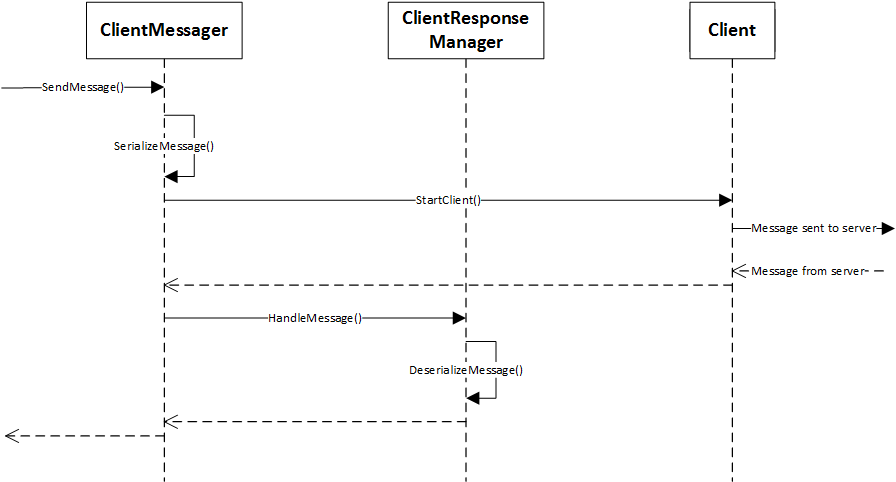
\includegraphics[width=0.9\linewidth]{figs/connection/ClientSequence.png}
	\caption{Client Sequence Diagram}
	\label{fig:ClientSequence}
\end{figure}

Et tilsvarende forløb i serveren er vist på figur~\ref{fig:ServerSequenceResponse}
\begin{figure}
	\centering
	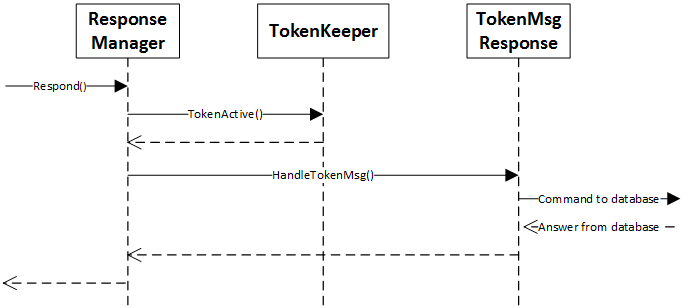
\includegraphics[width=0.9\linewidth]{figs/connection/ServerSequenceResponse.png}
	\caption{Server Sequence Diagram}
	\label{fig:ServerSequenceResponse}
\end{figure}